\documentclass{handout}

%\SetInstructor{Capt Steven Beyer}
\SetCourseTitle{ECE210: Introduction to Electrical and Computer Engineering}
\SetSemester{Spring 2019}
\SetHandoutTitle{Lab 11 - Obstacle Avoidance}

%\ShowAllBlanks

\usepackage[obeyspaces]{url}
\input{../arduinoLanguage.tex}

\graphicspath{{./figs/}}

%\showsoln \setsolncolor{red}

\lstset { %
	language=Arduino,
	frame=none,
	basicstyle=\footnotesize,
}

\begin{document}
	%	\footnotetext{Examples are abstracted from Tutorials Point, "Arduino", 2019, accessed Feb 18, 2019. [Online]. Available: https://www.tutorialspoint.com/arduino/index.htm}
	\maketitle
	
	\section{Objectives.} 
	\begin{enumerate}
		\item Become familiar with the Sharp GP2Y0A51SK0F Analog Distance Sensor.
		\item Utilize the Arduino to detect walls.
		\item Integrate the Distance Sensor with the DFECBot and program the DFECBot to avoid obstacles.
	\end{enumerate}
	
	\section{Materials.}
	\begin{enumerate}
		\item 3x Sharp GP2Y0A51SK0F Analog Distance Sensor
		\item USB Programming Cable
		\item DFECBot
	\end{enumerate}
	
	\section{Introduction.}
	
	\subsection{Sharp GP2Y0A51SK0F Analog Distance Sensor}
	The Sharp GP2Y0A51SK0F Analog Distance Sensor uses an infrared radiation (IR) reflectance sensor with an IR light-emitting diode (LED) and an IR sensitive phototransistor.\footnote{GP2Y0A51SK0F Datasheet, \url{https://www.pololu.com/file/0J845/GP2Y0A41SK0F.pdf.pdf}}Ensure your three sensors are wired per the below diagram.
	
	\begin{figure} [H]
		\centering
		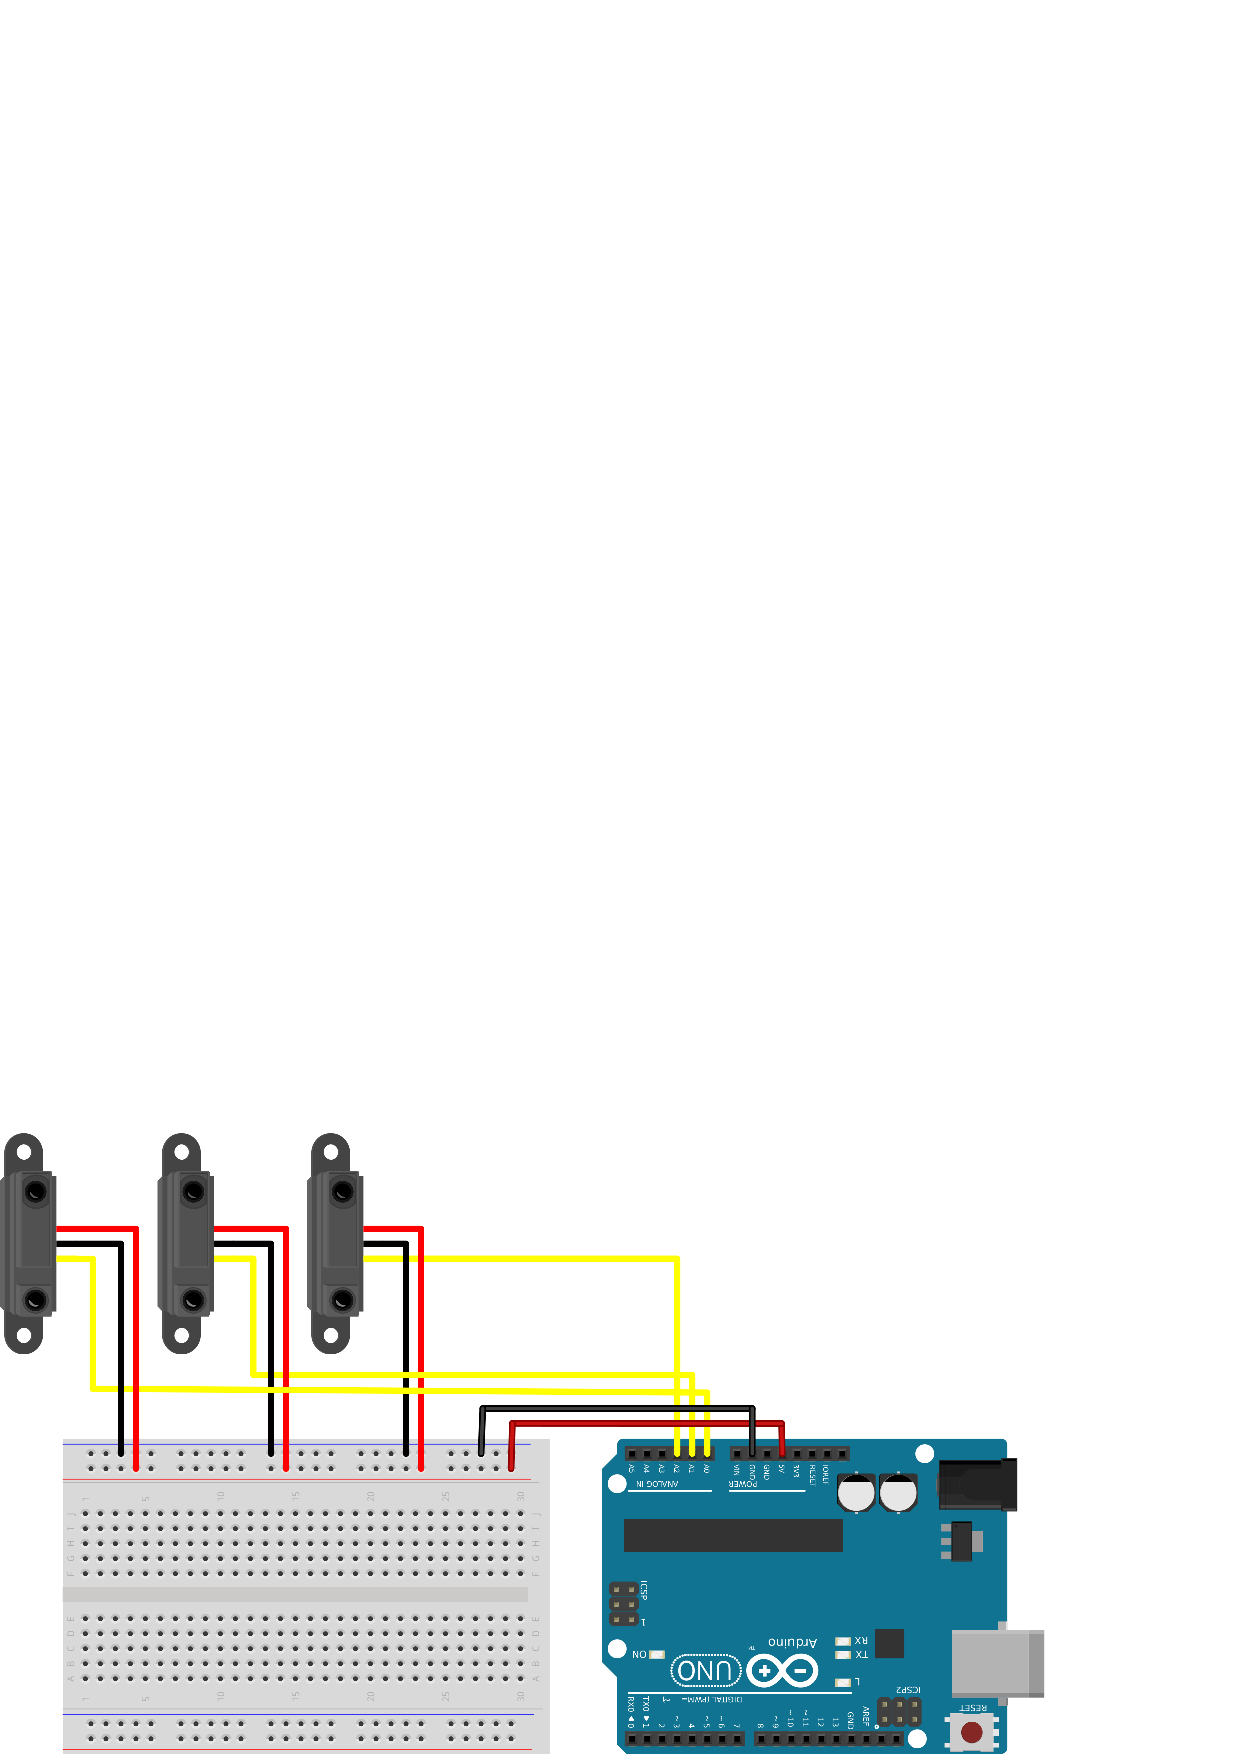
\includegraphics[width=.75\textwidth]{ir.jpg}
		\caption{Sharp GP2Y0A51SK0F Analog Distance Sensor Wiring Schematic}
		\label{Fig IR}
	\end{figure}

	\newpage
\clearpage
\pagebreak

	
	\subsection{Example Code}
	Copy the Arduino sketch folder \path{robot_wallfollowing}  from \textbf{Teams} (\path{Labs/robot_wallfollowing}). Open the \path{robot_wallfollowing.ino} sketch.
	
	\subsubsection{SharpDistanceSensor.h}
	The Arduino Sketch utilizes a library called SharpDistSensor. You need to install this library for the example code to work.
	\begin{enumerate}
		\item Click \textit{Tools} $\rightarrow$ \textit{Manage Libraries}
		\item Search for SharpDistSensor
		\item Select Install
	\end{enumerate}
	
	\subsubsection{robot\_wallfollowing.ino}
	This example Arduino Sketch provides code to read the values from the DFECBot's right Distance Sensor (see below example) and provides a distance value in $mm$.
	
	\begin{lstlisting}
		// Read distance (in mm) for each sensor
		unsigned int distR = sensorR.getDist() + OFFSET;
		Serial.print("Right: "); Serial.println(distR);
	\end{lstlisting}
	
	\section{Procedure}
	\textbf{Use the example code provided to code the DFECBot to do the following:}
		
	\begin{enumerate}
		\item Print the values from the DFECBot's center and left GP2Y0A51SK0F Analog Distance Sensor to the serial monitor.
		\item Use a ruler to confirm the accuracy of each distance sensor - the sensor should be fairly accurate between $3\ cm$ and $12\ cm$.
		\item Program the DFECBot to follow wall on right.
		\item Program the DFECBot to follow wall on left.
		\item Program the DFECBot to stay between two walls.
	\end{enumerate} 	
	{\large \textbf{\underline{HINT:}}} You should remove all print statements and delays when testing your wall following.
	\section{Notes on Proportional Controller:}
	
\end{document}
